\scanpage{27}\mspage{26}

\uline{Cor} Si $\mathrm{omb}(X)^\circ\cap\mathrm{omb}(Y)^\circ\neq\varnothing$, on a $X=Y$ / i.e. $X\neq Y\Rightarrow\mathrm{omb}(X)^\circ\cap\mathrm{omb}(Y)^\circ=\varnothing$

\margin{\unsure{$\mathrm{At}\,L\,1|\mathrm{At}_{L}\,1$}}
\[
\left|\begin{aligned}
&\uline{\text{ML 2}}\qquad \forall X\in M,\quad \mathrm{omb}(X)^\circ\neq\varnothing.\quad \text{i.e. }\exists x\in L,\quad x\overset{\circ}{\ll}X\\
&\uline{\text{ML 3}}\qquad \forall X\in M,\quad \text{les }\mathrm{omb}(Y)^\circ\quad(Y\in\widetilde X)\quad\text{recouvrent}\\
&\mathrm{omb}(X),\quad\text{i.e. }\deleted{\unsure{a}}\forall x\in L,\quad x\ll X,\quad\exists\deleted{\unsure{X}}Y\leq X,\ \text{avec }x\overset{\circ}{\ll}Y.
\end{aligned}\right.
\]
% slanted
\margin{$\mathrm{At}_{M}\,4$ a) pour $L$}

% slanted
\margin{ML 2 et ML 3 \deleted{\unsure{les|dès les}} signifient que les $\mathrm{omb}(Y)^\circ$ forment une \uline{partition} de $X$.}

\uline{NB} Par le cor. ci-dessus, cet $Y$ est unique.

Par le lemme, si \deleted{\unsure{$x\in|x\ll$}} $Y'\leq X$, et $x\ll Y'$, comme $x\in\mathrm{omb}(Y)^\circ\cap\mathrm{omb}(Y')$ \deleted{\unsure{alors}} on a $Y\leq Y'$ par le lemme, donc $Y'$ est le plus petit \unsure{élémt|élément} de $\widetilde X^x$. Plus généralement :

\deleted{\uline{Lemme 2} Soit $X,Y\in M$. $Y\ll X$. Alors}
\figure{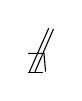
\begin{tikzpicture}[x=1cm,y=1cm]
\draw (0,.24)--(.20,.24)--(.22,.01);
\draw (0,0)--(.19,0);
\draw (.015,.005)--(.26,.56);
\draw (.085,.005)--(.32,.55);
\end{tikzpicture}}

On n'a pas jusqu'à présent, \unsure{utilisé|utiliser} la définition du \unsure{sous-ens|sous-ens.} $L$ de $M$, comme formé d'él. minimaux pour $\ll$. Donc \unsure{Tout|tout} marche avec un $L$ quelconque, pourvu qu'on suppose ML 2, ML 3 pour cet $L$. Si on \unsure{prenait|prend} $L=M$, ML 2 est trivial, ML 3 signifie que $\forall\deleted{\unsure{x\in}}X\in M$ et $Z\ll X$, $\exists Y\in\widetilde X$ tel que $Z\overset{\circ}{\ll}Y$, i.e. $\mathrm{At}_{M}\,4$ a)\unsure{''} (page 6). Mais il faudra dans ML 1 \deleted{\unsure{supposer que}} \inserted{généraliser}, en remplaçant $x$ par un $Z\inserted{\in M}$ quelconque.

Mais il devrait être possible de le prouver, via ML 3 \inserted{et ML 2} pour $L$, . L'idée est pour $\deleted{\unsure{Y}}Z\ll X$, de prendre $x\in L$, $x\overset{\circ}{\ll}Z$, \inserted{(ML \unsure{2|3})} et l'unique $Y\in\widetilde X$ tel que $x\overset{\circ}{\ll}Y$ (ML 3), et il \deleted{\unsure{po|pe}} faudrait prouver que $\deleted{\unsure{Y}}Z\overset{\circ}{\ll}\deleted{\unsure{Z}}Y$. Ceci se \unsure{décompose|discompose} en deux : si $x\ll Y\leq X$, \unsure{on a} $Z\ll Y$ et alors $x\overset{\circ}{\ll}Y$ \unsure{sss|ssi} $Z\overset{\circ}{\ll}Y$.
